%\documentclass[fleqn]{book}
\documentclass[11pt]{amsbook}

\usepackage[turkish]{babel}

%\usepackage{../HBSuerDemir}	% ------------------------
\usepackage{../Ceyhun}	% ------------------------
\usepackage{../amsTurkish}


\begin{document}
% ++++++++++++++++++++++++++++++++++++++
\hPage{147}
% ++++++++++++++++++++++++++++++++++++++
\setcounter{page}{147}
\setcounter{section}{3}
\setcounter{theorem}{2}
\setcounter{figure}{2}
\renewcommand{\theenumi}{\alph{enumi}}


Çevre, kesitleme, t-çevre ve t-kesitleme kavramlarını böylece
açıkladıktan sonra, bunlara yakın ilişkisi olan ikinci düzeyden
eşyapılılığı tanımlayabiliriz.
\begin{definition}
	Bir çizgeyi öbeklerine parçalamaya ya da çizgeye yalnız iki
	düğüm ile bağlı olan bir altçizyeyi ters yüz etmeye
	\textit{\underline{eşyapılılık işlemleri}} denir.
\end{definition}
Şekil 3.3'de Tanım 3'de açıklanan işlemlere örnekler verilmiştir.

\begin{figure}[h]
	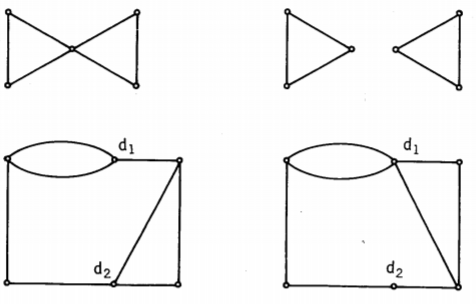
\includegraphics[scale=1.3]{images/ceyhun-147-fig01.png}
	\begin{caption}
		\enskip Eşyapılılık işlemleri 
		\begin{enumerate}
			\item Öbeklere ayrıma
			\item Altçizgenin d1, d2 düğümlerinde tersyüz edilmesi. 
		\end{enumerate}
	\end{caption}
\end{figure}



\end{document}